% Standalone Figure 1: horizontal overview of the dual-gate inspection pipeline.
% Authored near text width with ~8 mm arrow gutters so \linewidth placement
% keeps flow arrows visibly long. Vertical span opened (~1.35x prior height)
% so stage cards and outcome stack read taller when scaled to \linewidth.
% Compile: pdflatex fig-overview.tex
% Fonts: Computer Modern defaults (no lmodern / custom face).
\documentclass[10pt,border=5pt]{standalone}
\usepackage[T1]{fontenc}
\usepackage{amsmath,amssymb}
\usepackage{tikz}
\usetikzlibrary{arrows.meta,calc,positioning}

\definecolor{FAblue}{HTML}{2A78D6}
\definecolor{FAaqua}{HTML}{1BAF7A}
\definecolor{FAorange}{HTML}{EB6834}
\definecolor{FAviolet}{HTML}{4A3AA7}
\definecolor{FAred}{HTML}{E34948}
% Outcome colours follow the paper-wide figstyle mapping (C_PASS=Okabe-Ito
% green, C_DEFER=OI orange, refuse/reject=OI vermillion) so the schematic
% agrees with Figs 3, 10 and every data figure; previously PASS was blue and
% DEFER was green, which collided with the "good"-class green elsewhere.
\definecolor{FApass}{HTML}{009E73}
\definecolor{FAdefer}{HTML}{E69F00}
\definecolor{FAreject}{HTML}{D55E00}
\definecolor{FAyellow}{HTML}{EDA100}
\definecolor{FAink}{HTML}{0B0B0B}
\definecolor{FAinktwo}{HTML}{333333}
\definecolor{FAtick}{HTML}{666666}
\definecolor{FAgrid}{HTML}{E1E0D9}
\definecolor{FAsurface}{HTML}{FCFCFB}

\newcommand{\accentbar}[2]{%
  \fill[#2] ([xshift=0.4mm,yshift=-0.75mm]#1.north west)
    rectangle ([xshift=1.35mm,yshift=0.75mm]#1.south west);}
\newcommand{\camera}[2]{%
  \begin{scope}[shift={(#1,#2)},draw=FAblue,line width=0.5pt]
    \draw[rounded corners=0.25mm] (-2.1mm,-1.2mm) rectangle (2.1mm,1.2mm);
    \draw (-1.05mm,1.2mm) -- (-0.65mm,1.85mm) -- (0.65mm,1.85mm) -- (1.05mm,1.2mm);
    \draw (0,0) circle (0.85mm); \draw (0,0) circle (0.28mm);
  \end{scope}}
\newcommand{\gear}[2]{%
  \begin{scope}[shift={(#1,#2)},draw=FAaqua,line width=0.5pt]
    \foreach \a in {0,45,...,315}{\draw (\a:1.3mm) -- (\a:1.95mm);}
    \draw (0,0) circle (1.3mm); \draw (0,0) circle (0.45mm);
  \end{scope}}
\newcommand{\flooricon}[2]{%
  \begin{scope}[shift={(#1,#2)},draw=FAyellow,line width=0.5pt]
    \draw (-2.2mm,-1.35mm) -- (2.2mm,-1.35mm);
    \foreach \x/\y in {-1.7/-0.3,-0.5/0.7,0.6/0.05,1.7/1.2}{\fill[FAyellow] (\x mm,\y mm) circle (0.35mm);}
    \draw[densely dashed] (-2.2mm,1.65mm) -- (2.2mm,1.65mm);
  \end{scope}}
\newcommand{\routeicon}[2]{%
  \begin{scope}[shift={(#1,#2)},draw=FAviolet,line width=0.55pt]
    \draw (-2.2mm,0) -- (-0.45mm,0) -- (1.65mm,1.5mm);
    \draw (-0.45mm,0) -- (1.65mm,0); \draw (-0.45mm,0) -- (1.65mm,-1.5mm);
    \foreach \y in {1.5,0,-1.5}{\fill[FAviolet] (1.9mm,\y mm) circle (0.35mm);}
  \end{scope}}
\newcommand{\lockicon}[2]{%
  \begin{scope}[shift={(#1,#2)},draw=FAtick,line width=0.5pt]
    \draw[rounded corners=0.2mm] (-1.15mm,-1.2mm) rectangle (1.15mm,0.5mm);
    \draw (-0.7mm,0.5mm) arc (180:0:0.7mm and 0.9mm);
    \fill[FAtick] (0,-0.45mm) circle (0.22mm);
  \end{scope}}
\newcommand{\checkicon}[3]{\draw[#3,line width=0.65pt,shift={(#1,#2)}]
  (-1.15mm,0) -- (-0.2mm,-0.95mm) -- (1.25mm,1.1mm);}
\newcommand{\clockicon}[3]{%
  \begin{scope}[shift={(#1,#2)},draw=#3,line width=0.5pt]
    \draw (0,0) circle (1.25mm); \draw (0,0) -- (0,0.75mm); \draw (0,0) -- (0.7mm,-0.22mm);
  \end{scope}}
\newcommand{\crossicon}[3]{\draw[#3,line width=0.6pt,shift={(#1,#2)}]
  (-1.0mm,-1.0mm) -- (1.0mm,1.0mm) (-1.0mm,1.0mm) -- (1.0mm,-1.0mm);}

\begin{document}
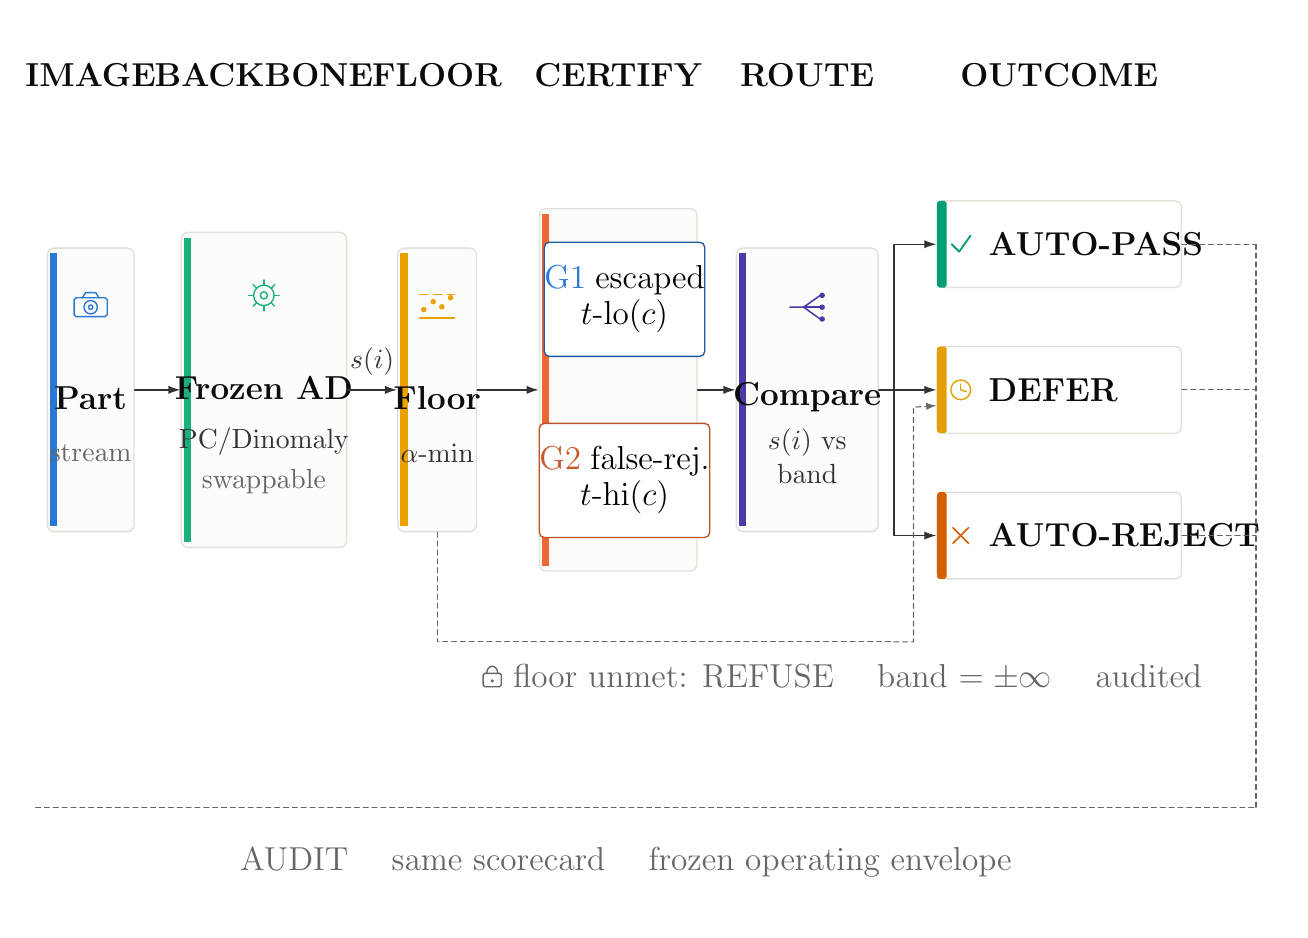
\begin{tikzpicture}[
  x=1mm,y=1mm,
  font=\normalsize,
  line cap=round,line join=round,
  >={Latex[length=1.55mm,width=1.05mm]},
  flow/.style={draw=FAinktwo,line width=0.5pt,-{Latex[length=1.55mm,width=1.05mm]}},
  control/.style={draw=FAtick,line width=0.42pt,dash pattern=on 1.8pt off 1.4pt},
  stage/.style={draw=FAgrid,line width=0.5pt,rounded corners=0.85mm,fill=FAsurface,
    align=center,inner sep=0pt},
  gate/.style={draw=FAgrid,line width=0.48pt,rounded corners=0.65mm,fill=white,
    align=center,inner sep=0pt},
  heading/.style={font=\bfseries\large,text=FAink},
  body/.style={font=\normalsize,text=FAinktwo},
  strong/.style={font=\bfseries\large,text=FAink},
  outcome/.style={font=\bfseries\large,text=FAink},
  note/.style={font=\large,text=FAtick,
    align=center,fill=white,inner xsep=0.6mm}
]

% Width held (~158 mm); height opened to ~118 mm (h/w ≈ 0.74 vs prior ~0.46)
% so \linewidth scaling yields a clearly taller figure.
\useasboundingbox (-1,-56) rectangle (158,56);

\node[heading] at (7,50) {IMAGE};
\node[heading] at (29,50) {BACKBONE};
\node[heading] at (51,50) {FLOOR};
\node[heading] at (74,50) {CERTIFY};
\node[heading] at (98,50) {ROUTE};
\node[heading] at (130,50) {OUTCOME};

\node[stage,minimum width=11mm,minimum height=36mm] (image) at (7,10) {};
\accentbar{image}{FAblue}
\camera{7}{20.5}
\node[strong] at (7,9.0) {Part};
\node[body,text=FAtick] at (7,2.0) {stream};

\node[stage,minimum width=21mm,minimum height=40mm] (backbone) at (29,10) {};
\accentbar{backbone}{FAaqua}
\gear{29}{22.0}
\node[strong] at (29,10.2) {Frozen AD};
\node[body] at (29,3.4) {PC/Dinomaly};
\node[body,text=FAtick] at (29,-1.6) {swappable};

\node[stage,minimum width=10mm,minimum height=36mm] (floor) at (51,10) {};
\accentbar{floor}{FAyellow}
\flooricon{51}{20.5}
\node[strong] at (51,9.0) {Floor};
\node[body] at (51,2.0) {$\alpha$-min};

% G1/G2 stacked; taller certify stage for vertical breathing room.
\node[stage,minimum width=20mm,minimum height=46mm] (certify) at (74,10) {};
\accentbar{certify}{FAorange}
\node[gate,draw=FAblue!75!black,minimum width=17mm,minimum height=14.5mm] (g1) at (74.8,21.5)
  {\textcolor{FAblue}{\large G1}~\large escaped\\[1.0pt]\large $t$-lo$(c)$};
\node[gate,draw=FAorange!80!black,minimum width=17mm,minimum height=14.5mm] (g2) at (74.8,-1.5)
  {\textcolor{FAorange!85!black}{\large G2}~\large false-rej.\\[1.0pt]\large $t$-hi$(c)$};

\node[stage,minimum width=18mm,minimum height=36mm] (route) at (98,10) {};
\accentbar{route}{FAviolet}
\routeicon{98}{20.5}
\node[strong] at (98,9.0) {Compare};
\node[body,align=center] at (98,1.6) {$s(i)$ vs\\band};

% Outcome stack: centers ~18 mm apart.
\foreach \name/\yy/\col in {pass/28.5/FApass,defer/10/FAdefer,reject/-8.5/FAreject}{
  \node[gate,minimum width=31mm,minimum height=11mm] (\name) at (130,\yy) {};
  \fill[\col,rounded corners=0.25mm]
    ([xshift=-15.5mm,yshift=5.5mm]\name.center) rectangle
    ([xshift=-14.3mm,yshift=-5.5mm]\name.center);
}
\checkicon{117.5}{28.5}{FApass}
\node[outcome,anchor=west] at (119.8,28.5) {AUTO-PASS};
\clockicon{117.5}{10}{FAdefer}
\node[outcome,anchor=west] at (119.8,10) {DEFER};
\crossicon{117.5}{-8.5}{FAreject}
\node[outcome,anchor=west] at (119.8,-8.5) {AUTO-REJECT};

\draw[flow] (image.east) -- (backbone.west);
\draw[flow] (backbone.east) -- (floor.west);
\node[body] at ($(backbone.east)!0.5!(floor.west)+(0,3.6)$) {$s(i)$};
\draw[flow] (floor.east) -- (certify.west);
\draw[flow] (certify.east) -- (route.west);
\coordinate (branch) at (109,10);
\draw[draw=FAinktwo,line width=0.5pt] (route.east) -- (branch);
\draw[flow] (branch) |- (pass.west);
\draw[flow] (branch) -- (defer.west);
\draw[flow] (branch) |- (reject.west);

% Refusal bus below outcome stack; audit lane further below.
\coordinate (refusebus) at (109,-22.0);
\draw[control] (floor.south) |- (refusebus);
\draw[control,-{Latex[length=1.3mm,width=0.9mm]}]
  (refusebus) -- (111.5,-22.0) -- (111.5,7.8) -- ([yshift=-2.0mm]defer.west);
\lockicon{58}{-26.5}
\node[note,anchor=west] at (60,-26.5)
  {floor unmet: REFUSE \quad band $=\pm\infty$ \quad audited};

\draw[control] (0,-43.0) -- (155,-43.0);
\draw[control] (155,-43.0) -- (155,28.5);
\foreach \arm in {pass,defer,reject}{\draw[control] (\arm.east) -- (155,0 |- \arm.east);}
\node[note] at (75,-50.0)
  {AUDIT \quad same scorecard \quad frozen operating envelope};

\end{tikzpicture}
\end{document}
